\documentclass[sisc-eikonal.tex]{subfiles}

\begin{document}

\section{Numerical Results}\label{sec:numerical-results} In this
section, we collect our numerical tests. We first test our factored
method on several different slowness functions with available exact
solutions for point source data. We also test our method on a linear
speed function (reciprocal of slowness) which has been shown to be
amenable to local factoring. For each quadrature rule described in
\cref{ssec:quadrature} (\texttt{mp0}, \texttt{mp1}, or \texttt{rhr}),
we have two 2D algorithms, \texttt{olim4} and \texttt{olim8},
corresponding to 4- and 8-point stencils, respectively. Since there is
no advantage in 2D, we don't apply the top-down or bottom-up
approaches. In 3D, we have three top-down algorithms: \texttt{olim6}
(group IVa), \texttt{olim18} (groups I, IVa, and IVb), and
\texttt{olim26} (group V). We also test the bottom-up algorithm
\texttt{olim3d} (see \cref{fig:hu-neighborhoods}).

\begin{figure}
  \centering
  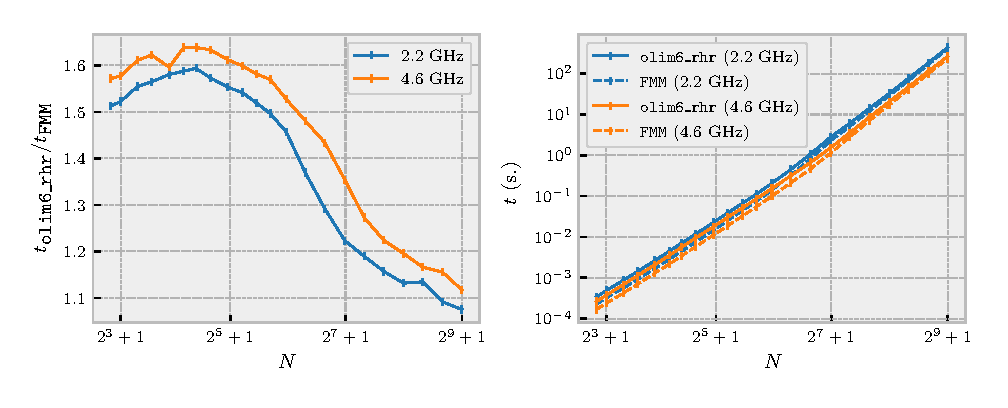
\includegraphics{speed-comparison.eps}%
  \vspace{-1.5em}
  \caption{To see how much of a slowdown we get by using
    \texttt{olim6\_rhr} instead of the standard fast marching method
    (noting that they compute the same solution), we compare runtimes
    on two different computers. The first (labeled ``2.2 GHz'') is a
    2015 MacBook Air with a 2.2 GHz Intel Core i7 CPU, 8 GB of 1600
    MHz DDR3 RAM, a 256 KiB L2 cache, and a 4 MiB L3 cache. The second
    (``4.6 GHz'') is a custom built workstation running Linux with a
    4.6 GHz Intel Core i7 CPU, 64 GB of 2133 MHz DDR4 RAM, a 1536 KiB
    L2 cache, and 12 MiB L3 cache. Both computers have L1 instruction
    caches and data caches that are each 32 KiB. From the plots, we
    can see that the difference in memory speeds has a significant
    impact on the relative slowdown.}\label{fig:speed-comparison}%
  \vspace{-1em}
  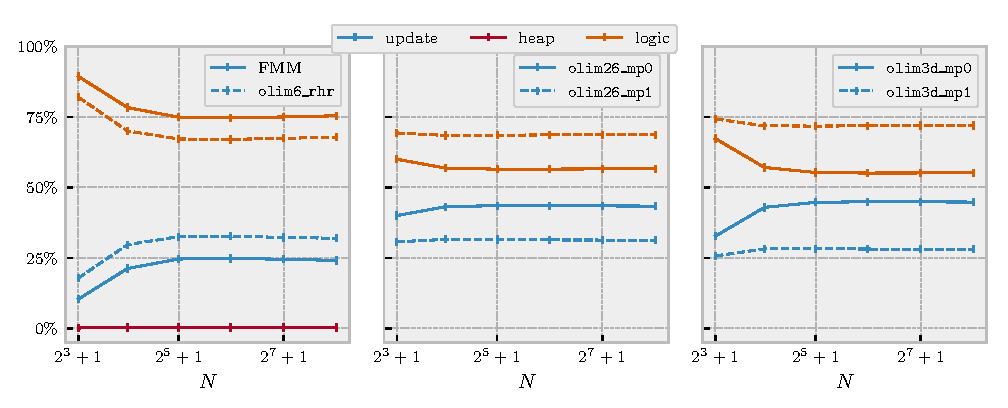
\includegraphics{tasks.eps}%
  \vspace{-0.5em}
  \caption{ The percentage of time spent doing different tasks. The
    ``update'' tasks and ``heap'' tasks are clearly defined, while the
    ``logic'' task contains a variety of things related to
    control-flow, finding neighbors, and memory movement---basically,
    the parts of \cref{alg:dijkstra-like} that don't clearly pertain
    to computing new $\hat{U}$ values or keeping \texttt{front}
    updated. From these plots, it is clear that memory speed plays a
    large role in determining efficiency. To some extent, even though
    the more complicated update procedures are slower, their slowness
    is hidden somewhat by memory latency as problem sizes grow. For
    some problem sizes, ``heap'' takes too little time, and is not
    picked up by the profiler.}\label{fig:tasks}
\end{figure}

\subsection{Implementation Notes}\label{ssec:impl-notes}

Before describing our numerical tests, we briefly comment on our
implementation and make some observations about its
performance. Different design decisions can be made when implementing
a Dijkstra-like algorithm which significantly affect its performance
characteristics. We list the following choices that we made in our
implementation:
\begin{itemize}
\item We precompute and cache all values of $s$ on the grid $\calG$,
  as opposed to reevaluating $s$ each time a value is needed. We chose
  to do this we assume that $s$ will generally be provided as gridded
  input data (consider, e.g., the shape from shading
  problem~\cite{kimmel2001optimal}, where the input data is an image).
\item We maintain the front using a priority queue implemented using a
  array-based binary heap, which is updated using the \texttt{sink}
  and \texttt{swim} functions described in Sedgewick and
  Wayne~\cite{sedgewick2011algorithms}.
\item The \texttt{front} data structure is stored as a dense grid of
  states: for each node in $p \in \calG$, we keep track of
  $p$\texttt{.state} for all time. Note that it is possible to
  maintain a sparse front which saves space but is slower to update.
\end{itemize}

We use a policy-based design~\cite{alexandrescu2001modern} written in
the C++ programmed language which makes heavy use of templates. This
allows us to conditionally compile different features and reuse logic
to implement different Dijkstra-like algorithms. In particular, we
implement the standard FMM~\cite{sethian1996fast} and make a direct
comparison between it and the ordered line integral method which it is
equivalent to, \texttt{olim6rhr} (see \cref{fig:speed-comparison}). We
have found that only a modest slowdown is incurred by using
\texttt{olim6rhr} for problems of moderate size. The disparity between
the two is greater for smaller problem sizes, which is due to cache
effects. We can expect the rest of our algorithms to incur a similarly
modest slowdown.

As a consequence of our design decisions, we note that our solvers
spend almost no time maintaing the front data structure. Using
Valgrind~\cite{nethercote2007valgrind}, we profiled running our solver
on the numerical tests below for different problem sizes and
categorized the resulting profile data. See \cref{fig:tasks}. The
``update'' task corresponds to time spent actually computing updates,
the ``logic'' task is a grab bag category for time spent on program
logic, and ``heap'' corresponds to updating the array-based heap which
implements \texttt{front}. Since the asymptotic complexity of the
``update'' and ``logic'' sections is $O(N)$ in the number of nodes,
and since ``heap'' is $O(N \log N)$, we can see from \cref{fig:tasks}
that since so little time is spent updating the heap, the algorithm's
runtime is better described as linear for practical problem sizes.

\subsection[Single point source]{Nonsymmetric slowness functions with
  a single point source}\label{ssec:point-source-problems}

Using \cref{eq:eikonal} directly, a simple recipe to create pairs of
slowness functions and solutions is to prescribe a solution $u$ and
compute $s(x) = \norm{\nabla u(x)}_2$. See
\cref{table:slowness-functions} for slowness function definitions. In
3D, the matrix we use for \texttt{s3} and \texttt{s4}
is:\begin{equation}
  A_{\texttt{s3}} = \begin{bmatrix}
    1 & \nicefrac{1}{4} & \nicefrac{1}{8} \\
    \nicefrac{1}{4} & 1 & \nicefrac{1}{4} \\
    \nicefrac{1}{8} & \nicefrac{1}{4} & 1
  \end{bmatrix} = A_{\texttt{s4}}^{1/2}
\end{equation}
Plots collecting our numerical results are contained in
\cref{fig:time-vs-error}. We include plots of relative
$\ell_\infty$ error plotted versus problem size and
time.

\begin{figure}
  \centering
  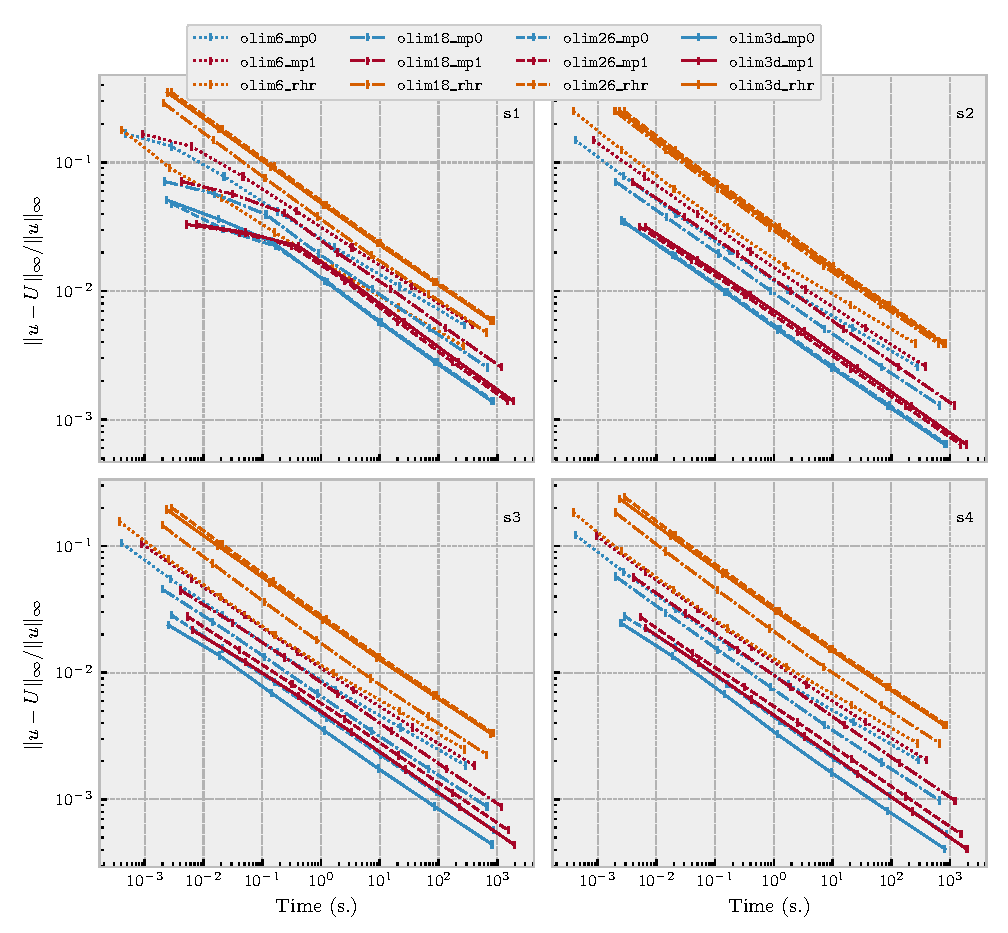
\includegraphics{time_vs_error_3d.eps}
  \caption{Relative $\ell_\infty$ error plotted against CPU runtime in
    seconds (see \cref{ssec:point-source-problems}). The domain is
    $\Omega = [-1, 1]^3$ discretized uniformly in each direction into
    $N = 2^p + 1$ points, where $p = 3, \hdots, 9$, so that there are
    $N^3$ points overall. The slowness functions used are listed in
    \cref{table:slowness-functions}.}\label{fig:time-vs-error}
  \begin{tabular}{cccc}
    Name & $u(x)$ & $s(x)$ \\
    \midrule
    \texttt{s1} & $\cos(r) + r - 1$ & $1 - \sin(r)$ \\
    \texttt{s2} & $r^2/2$ & $r$ \\
    \texttt{s3} & $S^\top A S$ & $\alpha\norm{\operatorname{diag}(C){(A + A^\top)}S}$ \\
    \texttt{s4} & $\tfrac{1}{2} x^\top A^{1/2} x$, where $A$ is symmetric positive definite & $\norm{x}_A = \sqrt{x^\top A x}$
  \end{tabular}
  \caption{Slowness functions used in point source tests. For these
    definitions, we assume that $x \in \Omega = [-1, 1]^3$, where
    $n = 3$. We also define $r = \norm{x}$,
    $S = (\sin(\alpha x_i))_{i=1}^3$, and
    $C = (\cos(\alpha x_i))_{i=1}^3$.}\label{table:slowness-functions}
\end{figure}

\subsection{A linear speed function}\label{ssec:slotnick}

\begin{figure}
  \centering
  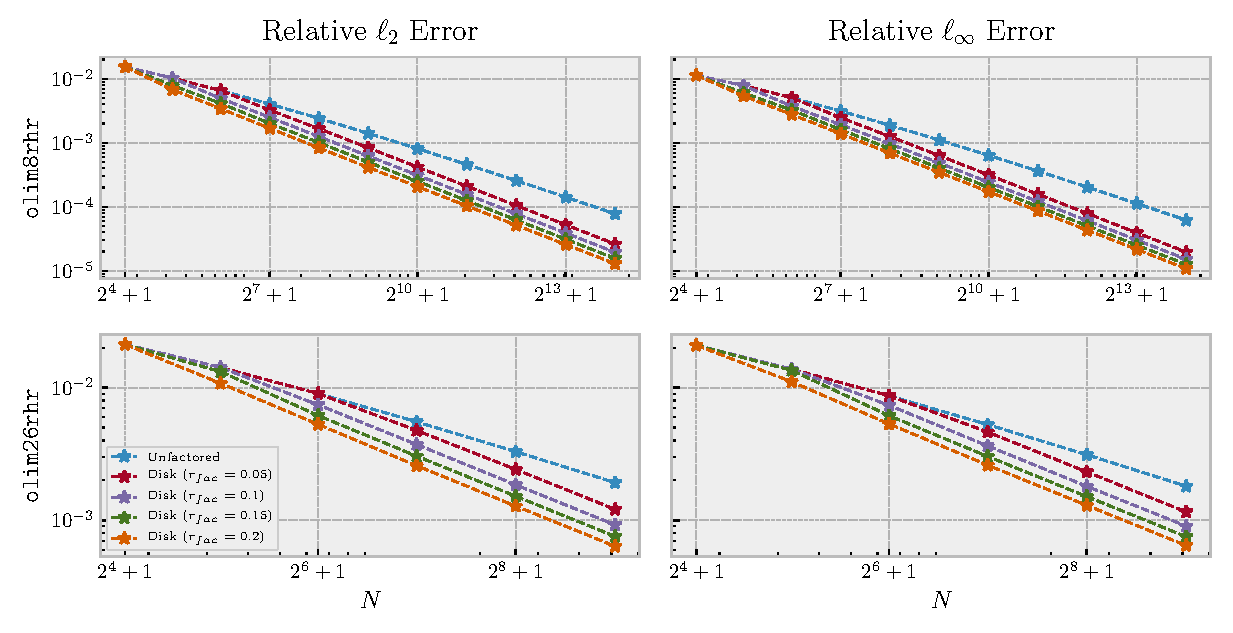
\includegraphics{factoring-error-example.eps}%
  \vspace{-1.4em}
  \caption{Comparing different ways of selecting factored nodes. For
    the test problem, $\Omega = [-1, 1]^n$, with $n = 2$ (first row)
    and $n = 3$ (second row). The domain is descretized into $N^3$
    nodes, where $N = 2^p + 1$, so that $h = 2/(N - 1)$. The slowness
    function is constant. For the 2D problem, \texttt{olim8rhr} is
    used; \texttt{olim26rhr} is used for the 3D problem. Solutions for
    the unfactored problem are plotted, along with solutions using a
    disk/sphere neighborhood with constant radius given by
    $\rfac = 0.05, 0.1, 0.15,
    0.2$.}\label{fig:factoring-error-example}
  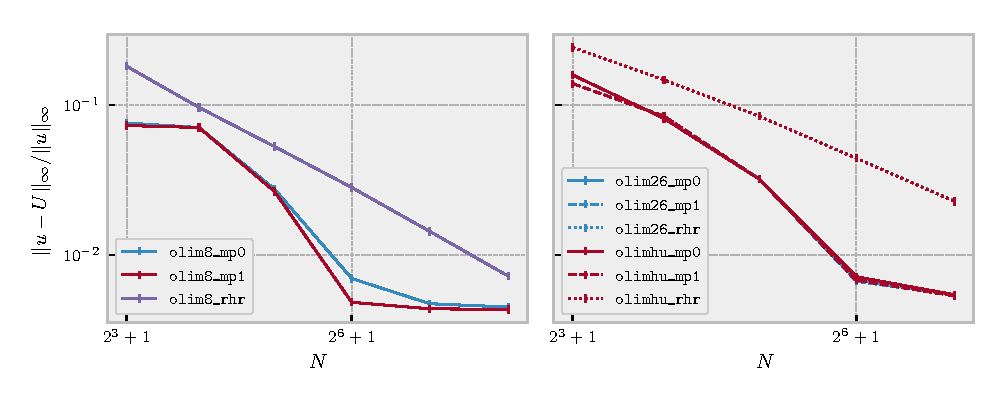
\includegraphics{qv_plots.eps}
  \caption{Numerical results for \cref{ssec:slotnick}. The relative
    $\ell_\infty$ error is plotted versus problem size $N = 2^p + 1$,
    where $p = 3, \hdots, 14$ in 2D and $p = 3, \hdots, 9$ in
    3D.}\label{fig:qv}
\end{figure}

We consider a problem that has an analytical ray tracing solution and
is used as a test problem elsewhere for solvers for the factored
eikonal
equation~\cite{slotnick1959lessons,fomel2009fast,qi2018corner}. For a
single point source at $x_i$ and a vector $v$, we define:
\begin{equation}
  \label{eq:slotnick-single-source}
  \frac{1}{s_i(x)} = \frac{1}{s_i} + v^\top {(x - x_i)},
\end{equation}
hence $s_i(x_i) = s_i$. The analytic solution to \cref{eq:eikonal} for a
single source and slowness function given by
\cref{eq:slotnick-single-source} is:
\begin{equation}
  \label{eq:slotnick-single-source-solution}
  u_i(x) = \frac{1}{\norm{v}} \cosh^{-1} \parens{1 + \frac{s_i}{2} s(x) \norm{v}^2 \norm{x - x_i}^2}.
\end{equation}
If we shift the point source from $x_i$ to another location $x_j$, we
find:
\begin{equation}
  \label{eq:slotnick-slowness-shift}
  \frac{1}{s_i(x)} = \frac{1}{s_i} + v^\top {(x - x_j + x_j - x_i)} = \frac{1}{s_i} + v^\top {(x_j - x_i)} + v^\top {(x - x_j)} = \frac{1}{s_i(x_j)} + v^\top {(x - x_j)}.
\end{equation}
Defining $s_j = s_i(x_j)$ and $s_j(x)$ from:
\begin{equation}
  \frac{1}{s_j(x)} = \frac{1}{s_j} + v^\top {(x - x_j)},
\end{equation}
we can see that $s_j(x_i) = s_i(x_j)$, that shifting the point source
from $x_i$ to $x_j$ is equivalent to changing the parameter $s_i$ to
$s_j$, and that $u_j(x)$ is defined analogously to
\cref{eq:slotnick-single-source-solution}. The solution for multiple
point sources $\set{x_i}$ is then given
by~\cite{fomel2009fast,qi2018corner}:
\begin{equation}
  u(x) = \min_i u_i(x).
\end{equation}

We compare relative $\ell_\infty$ errors in for each of our OLIMs in
2D and \texttt{olim26} and \texttt{olim3d} in 3D for this slowness
function. See \cref{fig:qv}.

\end{document}

%%% Local Variables:
%%% mode: latex
%%% TeX-master: "sisc-eikonal.tex"
%%% End:
